\documentclass[twoside, english, 11pt]{report}

\usepackage{babel}
\usepackage{graphicx}
\usepackage{times}
\usepackage{pifont}
\usepackage[margin=1in]{geometry} 
\usepackage{eurosym}
\usepackage{fancyhdr}
\usepackage[hidelinks]{hyperref}
\usepackage{framed}
\usepackage[thinlines]{easytable}
\usepackage{enumitem}
\usepackage{float}
\usepackage{lastpage}
\usepackage{titlesec}
\usepackage{caption}
\captionsetup{figurename=FIGURE}
\captionsetup{tablename=TABLE}
\titleformat{\chapter}
  {\normalfont\LARGE\bfseries}{\thechapter}{1em}{}
\titlespacing*{\chapter}{0pt}{3.5ex plus 1ex minus .2ex}{2.3ex plus .2ex}
\restylefloat{table}
\geometry{
 a4paper
 }
 

\pagestyle{fancy}
\fancyhf{}

%HEADER
%**************************************************************************************
\pagestyle{fancy}
\fancyhf{}
%**************************************************************************************
%\lfoot{Savonia UAS}		 	 
%\rfoot{Bachelor's Thesis} 
\chead{\thepage}
\renewcommand{\headrulewidth}{0pt}
%**************************************************************************************

\date{}
\setlength\parindent{0pt}

\begin{document}
\thispagestyle{empty}
\nopagebreak
\begin {flushleft}

\includegraphics{savonia.jpg}
\end{flushleft}
\begin {center}
\vspace{2.5in}\Huge Implementation of volume rendering in C\#\\ for LightningChart\\
\vspace{1cm}
 \LARGE Alexey Tukalo\\
 \vspace{0.5cm}
\large Bachelor's Thesis\\
\vspace{2.5in}
\today \hspace{0.5cm} \noindent\rule{4cm}{0.4pt}
\end{center}
\begin {flushleft}
\large Bachelor’s degree (UAS)
\end{flushleft}


\vspace{2.5in}

\date{\today}


\newpage
\setcounter{page}{1}
\setcounter{tocdepth}{2}
\newgeometry{inner=2cm,outer=4.3cm}

\begin{table*}[!h]
\begin{tabular}{| l | l | l | l |}
\multicolumn{2}{l}{\textbf{SAVONIA UNIVERSITY OF APPLIED SCIENCES}}&
\multicolumn{2}{r}{\textbf{THESIS}}\\
\multicolumn{4}{r}{\textbf{Abstract}}\\
\hline
\multicolumn{4}{|l|}{Field of Study}\\
\multicolumn{4}{|l|}{Technology, Communication and Transport}\\
\hline
\multicolumn{4}{|l|}{Degree Programme}\\
\multicolumn{4}{|l|}{Degree Programme in Information Technology}\\
\hline
\multicolumn{4}{|l|}{Author}\\
\multicolumn{4}{|l|}{Alexey Tukalo}\\
\hline
\multicolumn{4}{|l|}{Title of Thesis}\\
\multicolumn{4}{|l|}{Implementation of volume rendering in C\# for LightningChart}\\
\hline
Data & \today & Pages/Appendices & \pageref{LastPage}\\
\hline
\multicolumn{4}{|l|}{Supervisor}\\
\multicolumn{4}{|l|}{Arto Toppinen}\\
\hline
\multicolumn{4}{|l|}{Client Organization/Partners}\\
\multicolumn{4}{|l|}{Arction Oy}\\
\hline
\multicolumn{4}{|l|}{Abstract}\\
\multicolumn{4}{|l|}{ }\\
\multicolumn{4}{|p{14cm}|}{
Arctive Oy is a Finnish software company based in Kuopio. Their main product is LightningChart, the fastest C\# framework for the visualisation of scientific, engineering, trading and research data. The library contains a bunch of tools for visualisation of XY, 3D XYZ, smith and polar graphs, 3D pie/donut views, 3D objects.
}\\
\multicolumn{4}{|l|}{ }\\
\multicolumn{4}{|p{14cm}|}{
The company wanted to extend LightingChart's ability to render polygonal 3D models by volume rendering. It gives Arction an opportunity to attract new clients to use the product. As a result the framework will provide a unique possibility to render volume and polygonal models at the same visualisation.
}\\
\multicolumn{4}{|l|}{ }\\
\multicolumn{4}{|p{14cm}|}{
The project started from a literature research and comparison of different volume visualisation techniques. The best approach for the Arction's case was chosen and implemented it in the framework. The volume rendering engine is based on DirectX used together with C\# via SharpDX API and HLSL shader language for low level optimisation of complex calculations.
}\\
\multicolumn{4}{|l|}{ }\\
\multicolumn{4}{|p{14cm}|}{
The final chapter of the report contains an evaluation of the results and suggestion for a future development of the engine.
}\\
\multicolumn{4}{|l|}{ }\\
\hline
\multicolumn{4}{|l|}{Keywords}\\
\multicolumn{4}{|p{14cm}|}{
Visualisation, Ray Casting, 3D, C\#, LightningChart, DirectX, HLSL, Image Processing, Volume Rendering, Rendering
}\\
\hline
\end{tabular}
\end{table*}

\newpage

ACKNOWLEDGEMENTS\\

I am very thankful to Arction Oy for offering me an opportunity to take part in the development of the project. I really like the office atmosphere and freedom in terms of my working style and schedule allowed by the company.\\

My special thanks go to Mr. Pasi Toummainen, the CEO of the company, who expressed interest in my idea to extend the library by the volume rendering engine, gave me permission to work on the project and guided me especially in the very early part of the development process.\\

I am very grateful to Savonia UAS and especially lectures who used to teache me.  Moreover, I would like to say thank you to my supervisor of thesis and head of my Degree Programm, Mr. Arto Toppinen, Principal Lecturer, for his mentoring and support during the report writing stage of my work. \\

In addition, I would like to express my deepest gratitude to Karlsuruhe Institute of Technology, there I got the first experience with volume rendering via Ray Casting. I am especially grateful to Nicolas Tan, Jerome, who was my mentor during the part of my internship related to modification of Tomo Ray Caster 2 and to Aleksandr Lizin, the creator of the volume rendering engine based on WebGL.

\newpage

\tableofcontents

\chapter{INTRODUCTION}
This chapter contains brief information about the motivation behind volume rendering, my personal background in computer graphics especially volume rendering. It also introduces Acrtion as the owner of the project, explains the reasons for Arction's interest in the development, set requirements for the final product.
\section{Motivation}

Volume data is very common our day. An importance of the type of datasets will grow in the near future, because of development in the field of 3D data acquisition and possibilities to perform the visualisation of this type of information on a modern office workstation with an interactive frame rate.\\

Volume rendering is a process of multi-dimensional data visualisation into a two-dimensional image which gives the observer an opportunity to recognize meaningful insights in the original information. The technology allows us to represent 3 dimensions of the data via position in a 3D space and 3 more via color of the point.\\

The dataset can be captured by various numbers of technologies like: MRI\footnote{Magnetic resonance imaging}, CT\footnote{Computer tomography}, PET\footnote{Positron emission tomography}, USCT\footnote{Ultrasound computer tomography} or echolocation. They also can be produced by physical simulations, for example fluid dynamics. The set of technologies mentioned before demonstrates that volumetric information plays a big role in medicine. It is used for an advanced cancer detection, visualization of aneurisms and treatment planning. This kind of rendering is also very useful for non-destructive material testing via computer tomography or ultrasound. Geoseismic researches produce huge three-dimensional datasets. Their visualisations are used in an oil exploration and planning of the deposit development.\\
%http://www.labri.fr/perso/preuter/imageSynthesis/02-03/papers/volvistut.pdf

\section{Personal backgound}

The first experience in the visualisation of volumetric data was gained by me during my internship at the Institute of Data Processing and Electronics, which belongs to the Karlsruhe Institute of Technology (KIT). I was a part of the 3D Ultrasound Computer Tomography (USCT) team there. Their main goal is the development of a new methodology for early breast cancer detection. An algorithm for visualisation of five-dimensional datasets was developed by me during the work placement. In result the it was integrated into Tomo Ray Caster 2\footnote{JavaScript framework for the visualisation of 3D data, developed in Institute of Data Processing and Electronics} and USCT's edition of DICOM Viewer. An example of Tomo Ray Caster's output image is presented on figure \ref{fig:usc}.\\

\begin{figure}[!h]
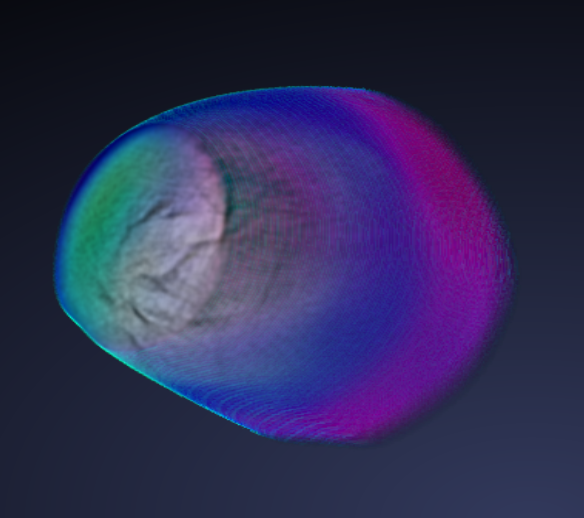
\includegraphics[scale=0.4]{img/usct1}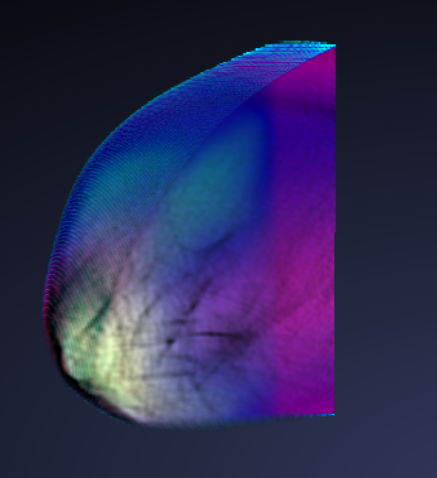
\includegraphics[scale=0.4335]{img/usct2}\\
\caption{Volume visualisation of breast phantom made by USCT\label{fig:usct}}
\end{figure}
%USCT VIS

The very first steps in modern computer graphics was made by me during the project. The first experience in work with WebGL was gained during customisation of the Tomo Ray Caster. GLSL as my first shader language was learned during the work. A lot of knowledge about image processing and scientific data visualisation, which became the basis for my thesis work was received by me at the workplacement.

%INTERNSHIP REPORT

\section{Arction Oy and Ligthning Chart}

Arction Oy is a Finnish software company based in Kuopio. Their team has a strong background in computer graphics and science. The main product of the company called LightningChart Ultimate. It is the fastest C\# library for scientific and engineering data visualisation. The library is capable to draw massive XY, Polar, Smith and 3D XYZ graphs, polygonal mesh models, surfaces, 3D pies/donuts and Geographic information. The library has an API for .NET WinForm and WPF applications, it is also possible to use it for a traditional Win32 C++ software development. The main advantage of the library is the fact that it is based on low-level DirectX graphics routines developed by Arction, then the most part of competitors use graphics routines which belongs to System.Windows.Media. Several example of the library's abilites are shown on the advetisment, figure \ref{fig:lchu}.\\
\begin{figure}[!h]
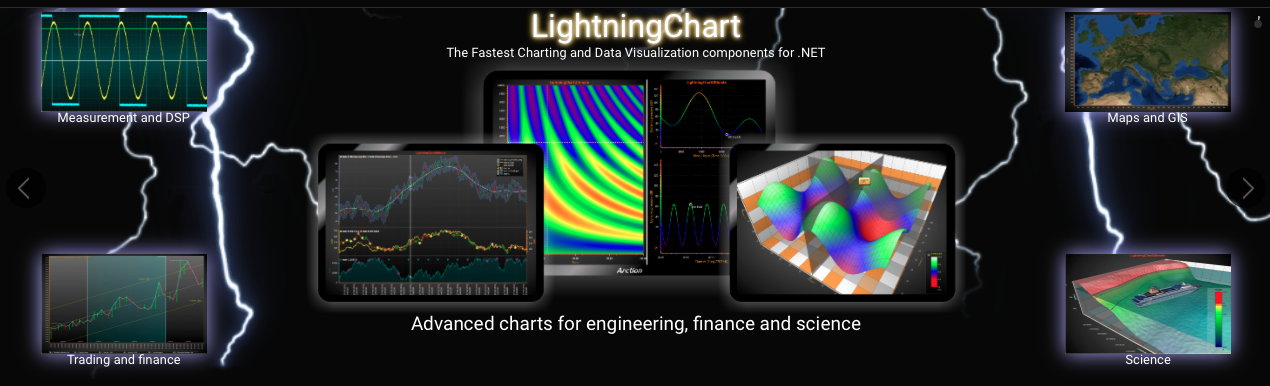
\includegraphics[scale=0.33]{img/lchu}\\
\caption{Example of LightningChart possibilities from the main page of Acrtion\label{fig:lchu}}
\end{figure}
%arction website

\section{Project Goals}

So, as it can be concluded from the previous section, LightningChart is a very advanced software for 3D rendering based on polygons and lines. That's why, an idea to extend it by the special rendering engine for visualisation of volumetric data was suggested by me to the CEO of the company. It will give Arction's clients the unique possibility to combine visualisation of volume datasets with a wide range of other 3D possibilities provided by the library. \\

The rendering engine must be able:
\begin{itemize} 
\item to render large multi-dimensional volumes with an interactive frame rate.
\item to move and rotate the model in the chart's space.
\item to provide clients with possibilities to apply windowing and thresholding to the initial dataset.
\item to render the model semi-transparent.
\end{itemize}

Basically, this tool will give end users possibilities to change the contrast and brightness of the model's visualisation for better recognition of tiny details and make areas, which are out off certain range, totally transparent. It will also reveal insights into the internal structure of the model to the user via semi-transparency.

\chapter{THEORY}

This chapter explains the theory behind the project. It should introduce the main concepts of computer graphics, specify the difference between polygonal mesh model and volume rendering. It also contains an overview of different volume rendering techniques with their advantages and disadvantages in terms of speed, final image quality, flexibility and other implementation issues.

\section{Rendering}

Visualisation of 3D object as 2D image called rendering. Usually, 2D image is based on pixels\footnote{a shortcut for picture element}. In case of a grayscale picture, it is a two-dimensional array and the value of the array elements represents the brightness of corresponding pixels on a screen. Configuration of colored images is dependent from a color model, the most popular one is RGB. It represents an image as three different grayscale pictures for three different colors called channels. In case of the RGB color model the images contain Red, Green and Blue values, sometimes it also keeps an informant about opacity and the channel called Alpha.\\

Color model is the mathematical abstraction which allows computers to calculate brightness of a corresponding point on the screen. RGB is the original one for modern computer graphics, because it represents colors in the way they are physically reproduced on screen. There are several other color models. They have their own advantages, for example, some of them gives us an advanced editing possibilities while others represent physical characteristic of different types of output devices like printers.\\

Multidimensional data can be represented in two different ways: as a surface and as volume. Future in this chapter, we are going to talk about these two concepts a little bit closer. We will highlight their advantage and disadvantages, common and uncommon features. Moreover, we are going to discuss an implementation detail of the techniques on modern hardware.

%https://www.artstation.com/artist/vidarrapp illustration


\section{Polygonal Rendering}

Today we are literally surrounded by the surface rendering based on polygonal mesh. The technology is used in computer games, design, cinema, science, engineering and etc. The technology is so popular that entire 3D graphic pipeline is built around the idea. That's why this type of visualization is easily accelerated by graphic cards.\\

\subsection{Vertexs}
Traditionally, 3D surfaces are constructed out of huge amount of polygons connected as a mesh. Due to simplicity, they usually have a triangular shape. It is possible to describe a triangle via list of three coordinates called vertices. The internal area of the shape filled with color during rasterization step. The color is calculated as dot product between the normal vector of the surface and the vector of light. An examples of wireframe and flat shading of the polygonal mesh model is demostrated on figure \ref{fig:mesh}
%http://people.csail.mit.edu/fredo/Depiction/1_Introduction/reviewGraphics.pdf

\begin{figure}[!h]
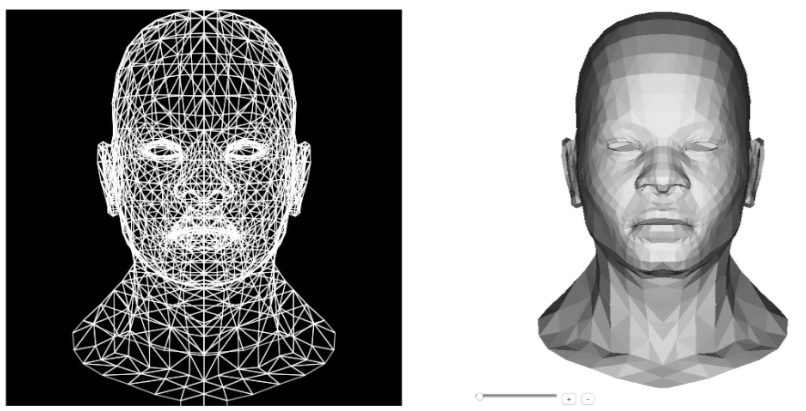
\includegraphics[scale=0.55]{img/mesh}\\
\caption{Wireframe and flat shading polygonal meshmodel\label{fig:mesh}}
\end{figure}

\subsection{Normals}
Surface normal vector of a triangle can be calculated as a cross product of two triangle's sides, but it will give an acceptable result only for very flat surfaces. That's why curve surfaces usually contain an additional normal vector for every vertex. They are able to significantly improve detailisation on the model. The information kept in them is used during shading and the tesselation of the model's geometry.\\

%http://www.emeyex.com/site/tuts/VertexNormals.pdf

\subsection{Textures}
Very small details can be added to the model via textures. It is specific 2D image which is used to sample high frequency information during rendering. The picture usually contains local color values, but it also can carry any information about normal vectors for a nice visualisation of very small structures on the surface. Textures are mapped to the surface via third parameter of vertex which is called texture coordinate. They keep any information about corresponding to this vector position in the 2D space of the image.\\

%http://www.dcs.ed.ac.uk/teaching/cs4/www/graphics/Web/advanced_ogl.pdf

\subsection{Redering process}
Position, scale, rotation of the object and perspective characteristics of the space is specified via matrixes $4\times4$. This kind of matrix allows to apply any kind of transformation possible in 3D space. Usually, three matrixes are applied to the object. The first one transfers an object to the world space coordinates, it specifies the position, rotation and scale of an original object in the world coordinate system. The next one is viewing matrix. It also takes in consideration position of camera and transforms the models to achieve desirable framing. The last matrix called projection. It applies perspective to the scene, in other word it defines an angle of view of the camera.\\
%http://www.opengl-tutorial.org/beginners-tutorials/tutorial-3-matrices/

%http://www.tutorialspoint.com/computer_graphics/3d_transformation.htm

Specific program called shader receives all the information together with a camera and light source positions, after that they are able to perform calculations needed to render the final image in accord with the goals of the visualisation. Usually, the calculations are produced by graphic card in a parallel way.

\section{Volume Rendering}

Volume data are composed out of voxels\footnote{volume element}. A voxel is simply a point in 3D space, which has a position and a color. Together gives us an opportunity to visualise up to six scalar parameters. There are two ways to render volumes. We are going to discuss about main principles, advantages and disadvantages of the technologies in this section.\\
%shear-warp paper 3

\subsection{Indirect}

The first one called indirect volume rendering. It is based on the idea that it is possible to extract surface out of the dataset during preprocessing and render the surface as a polygonal mesh. Several algorithms are invented for this application:
\begin{itemize}
\item Marching Cubes
\item Surface Tracking
\item Fourier Transfor Rendering
\end{itemize}
It is the oldest idea behind volume rendering and it has plenty of disadvantages:
\begin{itemize}
\item complex and slow preprocessing algorithms
\item can be inaccurate due to noise
\item sometimes does not able to generate an isosurface out of specific dataset, for example smoke
\item lose an information about an internal structure
\item need to repeat preprocessing to apply changes in a transfer function
\end{itemize}

But the algorithm is very popular for generation of medical illustrations, video or other static visualisation. The main advantage of the solution is that nicely preprocessed model can be easily rendered via well-known technique for 3D mesh model's rendering. They can be used even in very weak hardware.\\

Unfortunately, this technology is not suitable for our project, because it does not satisfy our requirements. First of all it is not acceptable for us to lose an internal structure and lose an opportunity to modify the transfer function runtime.
%http://www.forceflow.be/wp-content/uploads/2012/02/vr_overview.pdf

\subsection{Direct}
Direct volume rendering does not require any preprocessing. The data are visualised from an original dataset. It gives the algorithms an opportunity to modify a transfer function runtime. There are four most common technique for direct volume rendering algorithm, which will be discussed more detailed in this section in the future.\\

For an implementation of hardware acceleration for rendering process a volume data has to be loaded to the graphics cards. It is usually served as 3D texture or as set of 2D textures. For the optimization of a texture's buffer consumption, several slices can be collected to one huge texture map. 
%http://www.forceflow.be/wp-content/uploads/2012/02/vr_overview.pdf
\subsubsection{Texture-based}

As it was mentioned before the graphics pipeline of modern graphic cards is optimized for rendering of polygonal mesh models. So, volume rendering algorithms are forced to use this set of tools to achieve hardware acceleration. Texture-based volume rendering is the most straightforward way to achieve the aim.\

As it was already said textures are used to add tiny details to polygonal models. Any graphic library has an advanced set of tools for texture mapping, which can be used to this kind of volume rendering. The algorithm creates set of planes called proxy geometry. Transfer function maps the volumetric dataset on the proxy geometry. The final image is constructed out of the planes with mapped on them textures via Alpha-blending.\\

%http://http.developer.nvidia.com/GPUGems/gpugems_ch39.html
A proxy geometry can be created in two different ways. The first one called 2D texture-based rendering. In this case three different sets of planes are generated. All sets are generated perpendicular to a different direction in 3D space. This approach leads us to sudden jumps in image quality for different camera position and does not allow to change the sampling rate of the visualisation.\\
\begin{figure}[!h]
\centerline{
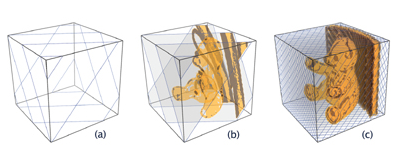
\includegraphics[scale=0.7]{img/texture-based}
}
\caption{a) an example of proxy geometry for 3D texture-based volume rendering a) Texture-based volume rendering with a lower sampling rate c) high sampling rate texture-based volume rendering\label{fig:text}}
\end{figure}
That's why the second way was invented. It is called 3D texture-based volume rendering. In this solution the algorithm creates only one set of planes which are always perpendicular to the camera and textures are mapped on them differently for the different camera position. The figure \ref{fig:text} shows an example of proxy geometry for 3D texture-based volume rendering, Texture-based volume rendering with a lower sampling rate and high sampling rate texture-based volume rendering.\\

It gets rid of an artifact of the first technique and allows to modify the sampling rate of the visualisation. The approach is the most popular direct volume rendering algorithm among medical software. But it has significant disadvantages against competitors. It is able to use, transfer function to emphasize or classify features of interest in the volume, while final blending is performed via Alpha-blending provided by DirectX API. It makes the approach less flexible than all other methods which provides more advanced tools for blending of sampled information.
%http://www.forceflow.be/wp-content/uploads/2012/02/vr_overview.pdf

\subsubsection{Ray Casting}

An image is produced by the algorithm throughout sampling of the volume along tracks of the rays which travel inside the dataset. A simple realisation of hardware acceleration of the approach require generation of boundaries for our volume. Usually they are represented by a cube.\\

Volume Ray Casting includes four simple steps:
\begin{itemize} \item An engine shoots a ray in a direction of observation for every point on a screen.
\item The ray travels through a scene and dataset.
\item A vector of the ray's track is calculated based on the position where the ray hits front and back faces of the cube.
\item The volume is downsampled along the ray track and color of the pixel is calculated out of collecting information in accordance with a Ray Function.
\end{itemize}
\begin{figure}[!h]
\centerline{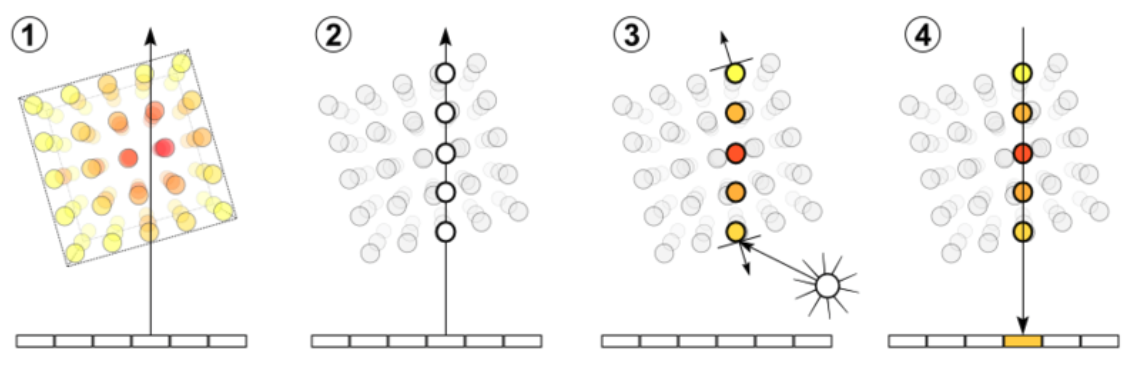
\includegraphics[scale=0.35]{img/rayCast}}
\caption{Ray Casting steps: 1) The ray is shot, 2) The ray travels through a scene and dataset. 3) Inlet and outlet position of the ray's track are detected 4) downsampling and the pixel's color calculation process}
\end{figure}

Ray Function is a core of the algorithm. Such a high level of flexibility is provided to the algorithm by the feature. It possesses an entire power of the technique, because it specifies the way how the data is combined.  It is very powerful tool for feature extraction, because it controls how color, opacity and gradient of isosurface are calculated by the engine. Transfer function and classification are also performed via Ray Function.\\

The algorithm has very high rendering quality without any additional artifacts. Due to the reason that every ray is calculated separately it is usually implemented in modern hardware focused on parallel calculations. The main problem of the algorithm is that rays usually do not hit the voxel's centers. In case of 3D space an interpolation is a very complex operation in terms of calculational expenses, which has to be performed to get a nice sampling.
\subsubsection{Splatting}

The technique was created to reduce interpolation expensis which were the main problem of Volume Ray Casting. The solution uses totally oposite aproach to reach the goal. Instead of sampling of the dataset by ray, the algorigthm projects the voxel to the image plane one by one. Of course the voxel porjections do not always fit excatly to pixels' grid of screen, but the problem is again solved by an interpolation, fortunately in this case the operation is much less expensive in term of calculation, becaus it is perfomed in 2D space. \\

The final pixel's color is calculated in a very similar way used by Ray Function, that is why the algorithm is as flexible as Volume Ray Casting. The main disadvantage of the approach is that some artifacts have contributed to the final image due to boxes overlap. It is also difficult to change the sampling rate of the approach. The issues make the algorithm less interesting for us. 

\subsubsection{Shear-warp}

As Splatting, the approach also tries to accelerate Ray Caster by solving of the interpolation issue, but it uses totally different way to illuminate the problem. Shear-warp has a very similar idea to the Volume Ray Casting. In some sense it is an optimization of the technique which makes rays always hit exactly in the center of the voxel.\\

The aim is achieved by the transformation of the volume data to sheared object space by translation and scaling of slices. After that an intermediate 2D image is produced by Ray Casting performed in the shared object space. The transformation brings some distortion to the output image. It is fixed at the last step of the algorithm called wrapping. The final image is the result of the transformation applied to the intermediate picture. The key difference between normal Ray Casting and Shear-Warp is shown in the figure \ref{fig:sw}.\\
\begin{figure}[!h]
\centerline{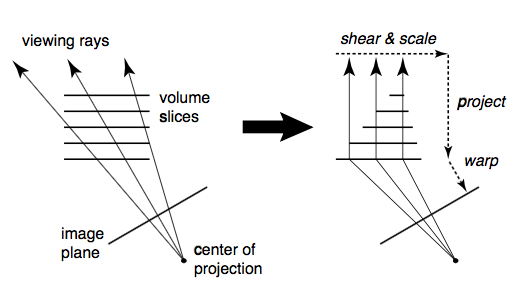
\includegraphics[scale=0.5]{img/shear-warp}}
\caption{(left)Ray Casting in world coorinates, (right)Ray Casting in shear object coordinates\label{fig:sw}}
\end{figure}
This solution gives us the fastest volume rendering process, but unfortunately the algorithm also suffers from several types of artifacts. Some of them are caused by an unevenness of sampling rate along different directions, others are produced by 2D transformation on wrapping stage.

\chapter{IMPLEMENTATION}
This chapter contains detailed explanation of the product implementation. It describes how the engine works, what kind of parts contains and which tools are used in it. The key step of the engine work is highlighted and explained in this chapter.\\

In accord with results of literature research, several the most common algorithms for volume rendering were compared and the most suitable approach was implemented as Volume Rendering Add-On of LigthinghChart Ultimate. One of the main requirements for the LightningChart's volume rendering engine is possible to combine volume and other 3D visualisation at the same chart space. Easy and accurate conversion between volume's and chart's coordinate systems is needed for this  purpose. Only volume ray caster and texture-based volume rendering can provide us with the feature. The algorithms keep entire visualisation inside the coordinate system of a proxy geometry. It is placed on the coordinate system of the chart. It means that the coordinates of volume model can be easily converted to the coordinates of the entire chart. Shear-warp and Splatting do not use any kind of proxy geometry, that is why they are not good solutuon for Arction's case.\\

Another important thing is implementation of rotation, scaling and transmission of the model in the chart space. As it was already mentioned the proxy geometry also makes it much easier. But this approach is not fully applicable for 3D Texture-based solution. In this approach slices always have to be perpendicular to the camera, that is why rotation has to be implemented in the process of texture mapping.\\

Finally, there are only two technologies. The final choice is Ray Casting, because it has better image quality than 2D Texture-based rendering. In addition, Texture-based volume rendering is less flexible than Volume Ray Casting.
\section{Tools}
This part of the chapter describes technologies used in the implementation of the project. It also gives a short explanation to their usage in the solution. The rendering engine has to become a part of LightningChart Ultimate. An integration with the library gives some restrictions in terms of a set of tools which can be used in the project and it plays a key role in technology selection.
\subsection{C\# and .NET}
C\# is a general purpose multi-paradigm programming language with strong types. It is created by Microsoft as the native language .NET Framework. Our days the language can be used for Web services, Windows desktop and mobile applications, computer games with several different game engines. In addition, Xamarin created set of tools for cross-platform C\# development.\\
%xamarin.com

In some since it contains constructions inspired by an object-oriented, imperative, functional and many other programming paradigms. The language belongs to C-like family, that is why the curly-brace syntax looks very similar to the C, C++, Java. C\# combines an advantages of Java and C++ in single, powerful and elegant way. It is more simple and safe than C++, but at the same times it has advanced features like: pointers arithmetics, enumerations, lambda expressions, structs, delegates and implicitly typed local variables. Even today when the most part of them are implemented in the last version of Java, C\# still is way more flexible.\\

Another advanced feature of C\# is  LINQ\footnote{Language-Integrated Query} expressions, it sets of functions for strongly-typed queries, which allows to write very short code in functional style for collection processing.\\

.NET framework contains applications run in a virtual execution system called the CLR\footnote{Common Language Runtime} and more than 4000 of classes which implements a wide range of useful functionalities. The runtime is able to execute an Intermediate Language, which is compiled from C\# or 20 other languages.
%https://msdn.microsoft.com/en-us/library/z1zx9t92.aspx

C\# is used in the project to reach as close integration with LightningChart Ultimate as it is possible. It performs loading and preprocessing of the dataset and management of visualisation process.

\subsection{DirectX 11}
DirectX is a C/C++ API\footnote{Application Programming Interface} for work with multimedia resources created by Microsoft for Windows and Xbox. It contains advanced tools for rendering of 2D and 3D graphic and sound management. Direct3D is a part of the library responsible for hardware accelerated rendering of 3D graphics. The tool is mainly focused on GPU accelerated rendering of polygonal mesh models.\\
%http://searchwindowsserver.techtarget.com/definition/DirectX
 \begin{figure}[!h]
\centerline{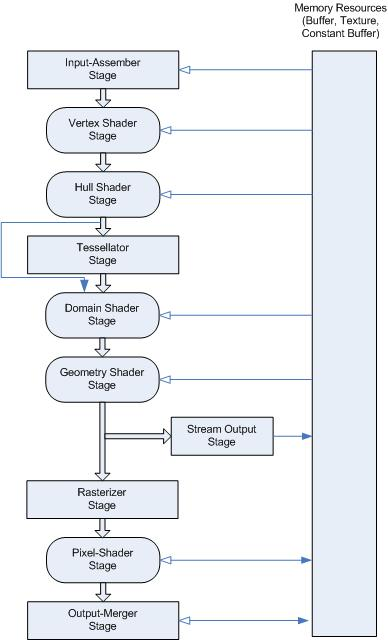
\includegraphics[scale=0.9]{img/pipeline}}
\caption{Flowchart of Direct3D 11 Graphics Pipeline\label{fig:pipeline}}
\end{figure}
\subsubsection{Rendering Pipeline}
The key concept of the library is a rendering pipeline. It is a very general term in computer graphics. The pipeline is a sequence of stages which receives an input data as a set of polygons, textures and variables, process the information step by step and generates the final image in the end.\\

Direct3D's pipeline has two types of steps:
\begin{itemize} 
\item Fixed-function - perform certain processing operation which can be customized up to some level via the API.
\item Programmable - processing is performed by the so called shader program. It is a function which is created by the developer and satisfies input and output parameters of the stage.
\end{itemize}

The graphics pipeline is shown on Figure \ref{fig:pipeline}. Boxes with rounded angles represent programmable stages and the other ones are fixed-functions. Let me explain every step of the pipeline more detailed:

\begin{itemize}
\item Input-Assembler Stage receive input information as a set of buffers and supply future to the pipeline. There are four types of buffers in Direct3D:
  \begin{itemize}
    \item Vertex Buffer is used to define the geometry of the object by a list of vertices. Every vertex has to follow Input Layout defined for the pipeline by the developer. It describes the vertex members: position and texture coordinates, color, value, normal etc. used in a particular application.
    \item Index Buffer conatins an order of vertexs as sequence of integer variables.
    \item Index Buffer contains an order of vertices as a sequence of integer variables.
    \item Constant Buffer provides pipeline with uniform variables data, like: transformation matrixes, position and directions of light sources, textures, and so on.
    %https://msdn.microsoft.com/en-us/library/windows/desktop/ff476898(v=vs.85).aspx
  \end{itemize}
\item Vertex Shader Stage is the first programmable stage of the pipeline. Vertices are read one by one and processed in accord with a Vertex Shader program which is supplied by the developer. For best performance the processing has to include every operation which can be performed on every vertex individually. The function is not able to destroy or create new vertex.

%книга
\item Hull Shader, Tessellator and Domain Shader stage are used together to achive tessellation\footnote{Process of mesh model's enchantment via automatic generation of additional polygons} of the mesh.
  \begin{itemize}
    \item The Hull Shader program includes two functions. The first one receive primitives and calculates tessellation factors out of the data. The second function is called once for every control point and creates them.
    %книга
    \item Tessellator uses data provided by Hull Shader and one of several algorithms to choose the best point to break of the current primitive into smaller polygons.
    \item Domain Shader uses an original information from Hull Shader together with results of the tessellator to generate the new vertex list.
  \end{itemize}
\item Geometry Shader receives several vertices at the same time and perform operations on them. An ability to add and remove points from pipeline makes the function extremely powerful and flexible tool. For example, it can easily turn single vertex to the polygon of even a set of polygons. It is able to pass geometry along the pipeline or to output stream.
\item Rasterization projects geometry to the final image and determines which pixels are covered by the polygons. It interpolates the verteces' atributes inside the primitives to get the pixels values for the area. It also perfoms depth and stencil tests.
\item Pixel shader is executed once for every pixel on the output target. It is supplied with an information from Resterizetion step and calculates per pixel data. Usually the texture sampling and high quality, lightning calculations are implemented with pixel shaders.
\item Output-Merge Stage uses pixel shader output together with depth/stencil information to generate the final image and write it in an appropriate way to render target.
\end{itemize}

It is worth to mention that a render target is not always represented by screen. Sometimes the output is stored in texture. For example the image can be loaded again to the graphic card. It can be used to get some pre-calculated previously information. The technique, called multi-pass rendering.

%https://msdn.microsoft.com/en-us/library/windows/desktop/ff476882(v=vs.85).aspx
\subsubsection{HLSL}
There are two ways of rendering pipeline customization. Fixed-functions behavior can be modified by the API. A flexibility of programmable stages  is organized via a special type of programming languages called Shader Languages. Direct3D's realisation of shared language called HLSL\footnote{High Level Shader Language}.\\

The language is basically significantly modified version of C. The language does not support an advanced features like pointer's arithmetics and dynamic memory allocation, but the syntax is still understandable for C developers. It extends C syntax by classes, several new data types, buffers, semantics and huge library of useful for shared development functions. There are vector, matrix and 1D-3D texture data types which are very useful for processing of 3D primitives. As it was already mentioned buffers are used to supply pipeline with data. Sematics contains metadata which is related to data exchange among fixed-function and programmable stages of the pipeline.
\subsection{SharpDX}

As it was already mentioned DirectX is C++ library, so it is not possible to use directly from C\#. The problem is solved by SharpDX. It is an open-source C\# wrapper for the original DirectX API. It plays role of bridge between API and .NET. As a result, developers are able to manipulate with the functional of the API from C\#.\\
%http://sharpdx.org
Every feature of the API is implemented in a very natural way. That is why a huge amount of tutorials and example available for the original C++ API can be easily translated to C\# and SharpDX. Even original documentation is still useable for SharpDX developers.

\subsection{LightningChart Ultimate}

LightningChart Ultimate is the fastest C\# library for scientific and engineering data visualisation. It is able to draw massive XY, Polar, Smith and 3D XYZ graphs, polygonal mesh models, surfaces, 3D pies/donuts and Geographic information. 

\begin{figure}[!h]
\centerline{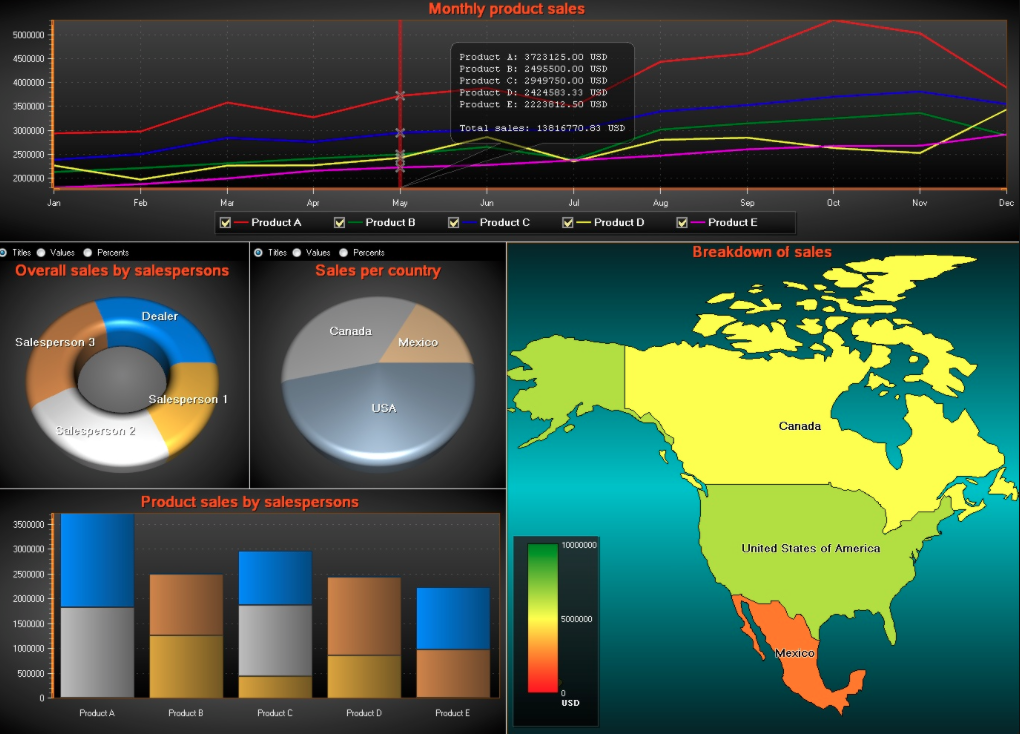
\includegraphics[scale=0.4]{img/chart}}
\caption{Some of LightningChart Examples}
\end{figure}

The library has an API for .NET WinForm and WPF applications, it is also possible to use it for a traditional Win32 C++ software development. The main advantage of the library is the fact that it is based on low-level DirectX graphics routines developed by Arction, then the most part of competitors use graphics routines which belong to System.Windows.Media.\\

An integration with LightningChart has several advantages and disadvantages. On one hand, it plays main role in terms of tool selection for project implementation, because deep enough integration can be achieved only via usage of a exactly same set of technologies. It also forces the volume rendering engine to follow similar architecture. Moreover, LightningChart is a commercial software package. That is why any external dependencies have to be avoided as much as it is possible. It means that even open-source libraries cannot be used without extremely important reason.\\
%http://arction.com/products_lc_ultimate_sdk

On the another hand, an abilities of LightningChart to draw 3D polygonal mesh models make the development much more simple. The library is able to rotate, scale and move the models around chart's space, so the functionality can be easily applied to proxy geometry. As a result the features are implemented without almost any development from the side of the volume rendering engine. In addition, it is a huge advantage for clients, because the volume and mesh 3D models can be visualized at the same chart in the same coordinate system. It provides them with really a unique and powerful opportunity for complex 3D visualisations.

\section{Visualisation process}

This section of the paper explains main principles and implementation details of the project. It describes the main challenges and explains how they were solved during development of the rendering engine.

\subsection{Loading and preprocessing of dataset}
The most common way of volume data distribution is a collection of 2D slices. The 2D slices are just images in common formats. Sometimes they can be represented as set of DICOM\footnote{Digital Imaging and Communications in Medicine} files. In this case they contain metadata of the studies together with embedded pictures. Volumes can also be distributed at table of original values. The table usually is part of RAW file which also contains some meta information. Actually, RAW is several different formats with common name. More detailed specification of every single realisation depends from a machine which performed the data acquisition.\\
\begin{figure}[!h]
\centerline{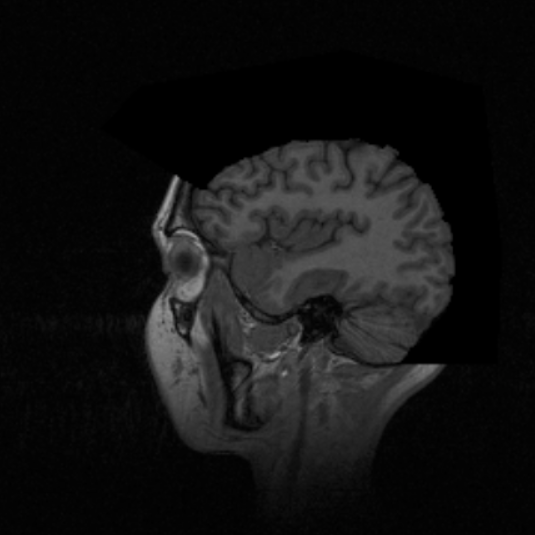
\includegraphics[scale = 0.35]{img/slice}}
\caption{Example of slice from Volume dataset.\label{fig:slice}}
\end{figure}
Unfortunately, the current implementation of the volume rendering engine supports only a first approach, because slice-based data is easier to get. Specific software can convert DICOM slices to the picture formats supported by .NET like *. JPEG, *. TIFF and *. PNG. RAW volume data files can be converted to *. CSV files, but due to the reason that there are many different specifications of the the extension it is very difficult to find the software.\\

.NET tools for file handling are responsible for loading of images in supported by the framework formats. The slices are loaded into the memory from specified folder as an array of bitmaps in the same order they are already stored. An example of a slice is shown on Figure \label{fig:slice}. DirectX 11 also supports 3D textures, but the approach was not used in the engine, because the feature is not supported by DirectX 9. Arction wanted to have an opportunity to port the volume engine to DirectX 9 quickly, if it would be needed. \\

\begin{figure}[!h]
\centerline{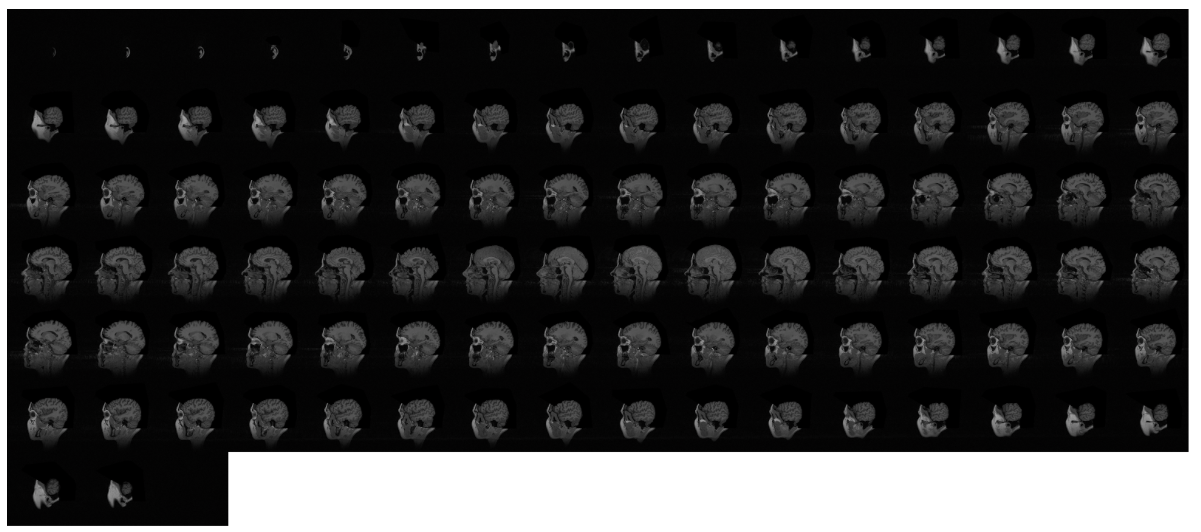
\includegraphics[scale = 0.35]{img/map}}
\caption{An example of slice map\label{fig:map}}
\end{figure}
Constant buffer has a limited amount of available slots for texture. Slices usually have a very low resolution so it is not efficient to load them one by one. For an optimization of of consumption of the buffers, an array of slices is mapped to the big texture map. The map contains slices mapped from left to right in accord with an array index, look Figure \label{fig:map}. A bitmap processing is accelerated via pointer arithmetic, but anyway it requires some time. That is why the engine is also able to load preprocessed texture map for quicker start of visualisation. \\

\begin{table*}[!h]
 \begin{center}
    \begin{tabular}{ c  c }
    \multicolumn{2}{l}{TABLE 3.1: Maximum size of a texture for different feature levels \label{tab:level}}\\
    Feature level & Maximum size of a texture\\
    \hline
    9\_2 & 2048\\
    9\_3 & 4096\\
    10\_0 & 8192\\
    10\_1 & 8192\\
    11\_0 & 16384\\
    11\_1 & 16384\\
    12\_0 & 16384\\
    \end{tabular}

  \end{center}
\end{table*}
DirectX has a limitation in terms of the biggest available texture size, which can be loaded to the graphic card. The value depends from feature level of the graphic card, look table 3.1. Feature level defines the functionality supported by the graphic card. Usually, modern graphic cards have at least 11\_0. It means that they support up to 16 384 pixels per side. Such a big texture can keep the volume dataset with more than 600 voxel long in every dimension. It is possible to render even bigger models, because several texture maps can be generated if it is not possible to fit enter data into a single one.\\
%https://msdn.microsoft.com/en-us/library/windows/desktop/ff476876(v=vs.85).aspx

\subsection{Multi-pass rendering}

Possibility to render a scene in several steps makes rendering pipeline especially flexible. The technique, called the Multi-pass rendering. Sometimes it is more efficient to render a scene in several steps. Multi-pass rendering is based on an idea that every step except the last one outputs the result of performing calculation to to texture. The final pass samples information from the set of textures and generates the output image.\\

Deferred rendering is one of the most popular realization of the idea. The technology is created for rendering of scenes with large amount of dynamic lights. Traditionally, this kind of functionality requires a complex set of shaders. Multi-pass approach breaks the process to smaller pieces and performs the calculations separately for every step. It allows to simplify an architecture of rendering framework. It can also give an opportunity to apply GPU acceleration to some parts of rendering algorithm which used to be executed on CPU before.\\

Our volume ray caster is also going to get some advantages from multi-pass rendering. In case of this solution, it has only two passes. It allows the algorithm to determine vectors of the sampling ray in the volume coordinate system without any additional mathematical calculations. It means that entire rendering pipeline of the engine contains two typical rendering pipelines. The first one generates texture which contains an important information for rendering of the final image at the second pass. Both passes use only vertex and pixel shader programs.

\subsection{First pass}

At this step rendering engine has to generate texture which keeps an information about the exit position of sampling rays. For this reason front-face culling mode of Direct3D has to be turned on. It makes the library to draw only polygons which are normally not visualised, because their front side looks in an opposite to the screen's direction.\\

An input of the first pass contains only set of vertices of the boundaries of the dataset, constant buffers for slice range clipping and matrices for calculation of the vertex position of the chart space. The boundaries are always represented by a cube. The cube contains 8 vertices calculated on C\# according with the required size of the volume model. Constant buffer is represented by two Vector3 variables, one of them contains the number of minimal slices for every direction and another one keeps an information about maximal boundaries. We also have three traditional for 3D graphic Matrixes: World, View, and Projection Coordinate. This matrix has unique values for every object and allows to calculate desirable position, scale and rotation of the object in screen coordinates.\\

The Vertex Shader of the first pass calculates positions of the cube vertices in accord with a clipping range buffer. After that matrixes are applied to transform the geometry to the screen coordinates. Internal coordinates of the dataset are calculated out an original position of vertex. They are represented by Vector3, with value range from 0 to 1 along every axis and stored as texture coordinates.\\

The Pixel Shader represents the coordinates as color. X coordinate is stored in the red channel, Y one is stored in the green channel and Z coordinates is stored as blue value. The final result of the first pass is demonstrated on Figure \ref{fig:first}.
\begin{figure}[!h]
\centerline{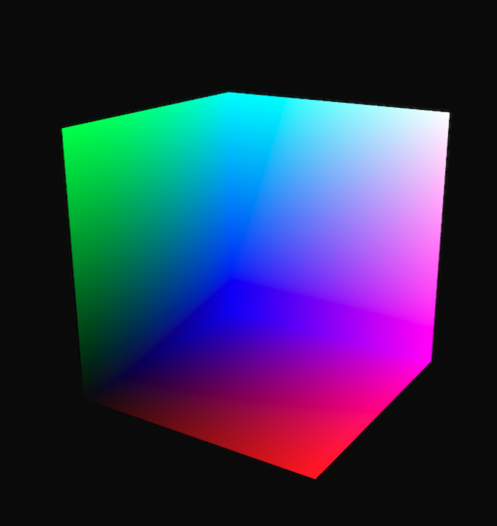
\includegraphics[scale = 0.5]{img/first}}
\caption{The first pass output\label{fig:first}}
\end{figure}

\subsection{Second pass}

At this pass the engine has to calculate the vector of sampling ray displacement through the dataset. The input coordinates of the rays are needed for the calculation that is why the default culling mode has to be restored. The coordinates are defined by position where the rays hit at the front sides of the cube's planes. The input of the pipeline has a set of vertices, matrices, an original dataset represented as a texture map, texture created at the first pass, buffers with slice range, contrast, brightness and threshold setting.\\
\begin{figure}[!h]
\centerline{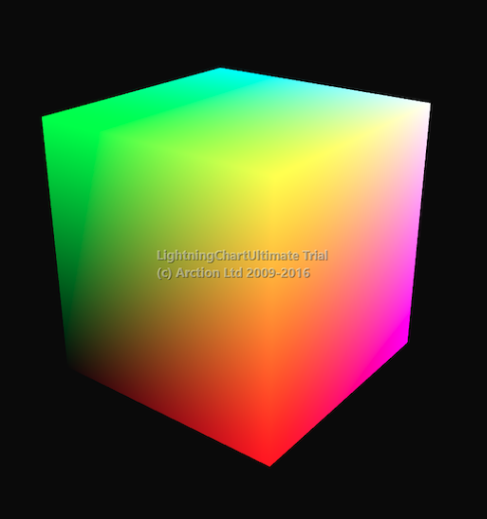
\includegraphics[scale = 0.5]{img/second}}
\caption{Coordinates of hit points.\label{fig:second}}
\end{figure}

Second pass has exactly same vertex shader with the first one, but due to changes in clipping mode it outputs the inlet points of sampling rays.  Figure \ref{fig:second} shows them in the same way it was done on the first pass.\\

The pixel shader subtracts the input coordinates from output ones. The input coordinates are calculated at the vertex shader of the second pass. The output coordinates keep positions where rays hit the back side of the cube. They are sampled from the texture generated at the first pass. The operation result is the vector of the ray's track. The tracks are visualized as colors on the figure \ref{fig:final} The vector is divided by sampling rate to get step vector.
\begin{figure}[!h]
\centerline{
\includegraphics[scale = 0.5]{img/final}}
\caption{The visualisation of the sampling rays vectors' tracks \label{fig:final}}
\end{figure}
Actual volume sampling is performed by for loop. It starts from the hit point of the ray and adds the step vector every intention to get coordinates of the new sampling point. The data are sampled out of volume by a function which calculates the corresponding position on the texture map.\\

It calculates the nearest slice corresponding to the Z position. After that it checks how many full rows are included in the value and what is the column number of the rest. Values from two closest slices can be interpolated to get a smoother result. Handling of the information depends from Ray Function.\\

\subsubsection{Empty space skipping}

The most part of volume dataset is represented by an empty space. Empty space does not contain any important information, usually it is represented by pixel with a very low value per each channel. In our case a voxel is classified as empty one if its values are out of an acceptable range for all of channels. There is a huge amount of rays which travels through arrays which contains only empty space. In addition there are areas with an empty space in front and behind the model. The optimization has to prevent high resolution downsampling of this regions.\\

Due to the realisation of the technique, the sampling is broken down into two steps. At the first step ray travels through dataset with a very low sampling rate. It saves positions of the first and the last non-empty voxels which is met by the ray. After that the second ray starts a one low resolution sampling rate step vector earlier than the position of the first non-empty voxel. It stops a one low resolution sampling rate step vector after the very last non-emtpy voxel detected by the first ray. The process is shown on figure \ref{fig:empty}. The ray with low sampling resolution can skip some part of non-empty voxels between sampling position. In this case actual border of the shape can be a little bit further or closer.  Possible artifacts are prevented by two low resolution sampling rate steps which is added in front and behind the model.\\

\begin{figure}[!h]
\centerline{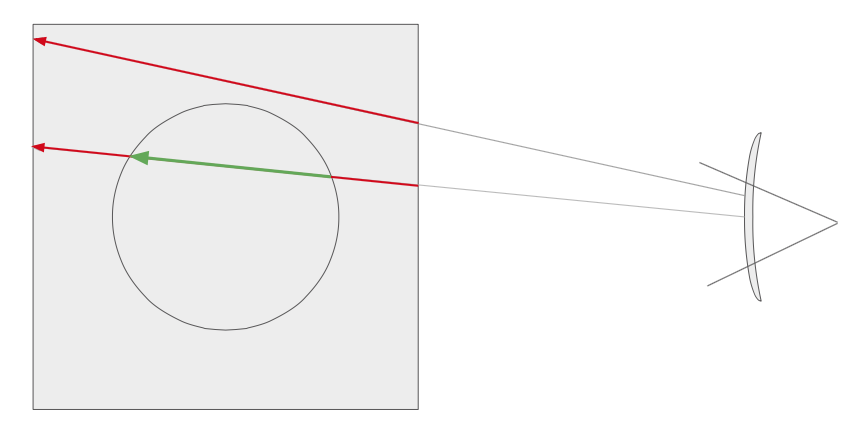
\includegraphics[scale = 0.5]{img/empty}}
\caption{Red arrows represents the low sampling rate ray. Green demonstrates high resolution sampling one.\label{fig:empty}}
\end{figure}

High and low resolution sampling rates are specified by constant buffer. High sampling rate determines rendering quality. An optimal quality is reached, then it match an amount of voxels in the longest dimension, because it allows to perform uniform sampling of the entire dataset and collect all information stored inside. Lower resolution sampling can only be defined via experiment. Too small, low resolution of sampling rate can contribute some artifact to the final picture. It is a trade of quality and frame rate. The right value has to keep an interactive frame rate and unnoticeable level of artifacts.


\subsubsection{Ray function}
Ray function determines the way how the sampled data are combined. A different ray functions allow to extract different features out of the dataset. Two the most common ray functions are implemented in our rendering engine.\\

Accumulation function uses alpha-compositing to collect as much data as it is possible. The visualisation which are produced by this technique looks like semi-transparent gel. Ray function implementation is represented by for-loops, which runs from 0 to the number of samples which is need to perform sampling of the region in according with desirable sampling rate. Every iteration contains several steps:
\begin{itemize}
\item The voxel is sampled out of the texture map.
\item The validation of voxels value is performed by if-statement. It checks that every channel is in its personal threshold range. If the voxel is empty next four steps have to be skipped.
\item The alpha is calculated in accordance with an equation:
\begin{equation} \label{eq:alpha}
\alpha_{output} = \alpha \times opacity \times \frac {1}{{sampling\ rate}}
\end{equation}

\item The colors are calculated in accordance with an equation:
\begin{equation} \label{eq:color}
color_{output} = (1 - \alpha_{accomulation}) \times (color + brighness) \times contrast  \times \alpha
\end{equation}\\

$\alpha_{accomulation}$ contains previously accumulated alpha values. Brightness and contrast are supplied by constant buffers and used to perform dynamic range correction.
\item After that the colors and alpha values are added to the corresponding variables which keep a previously accumulated information.
\item If-statement checks that alpha is not oversaturated. The ray has to be terminated in this case, due to performance optimization.
\item Step vector is added to reach next sampling position.
\end{itemize}

An example of images produced by an accumulation function is demonstrated in figure \ref{fig:accum}. \\

\begin{figure}[!h]
\centerline{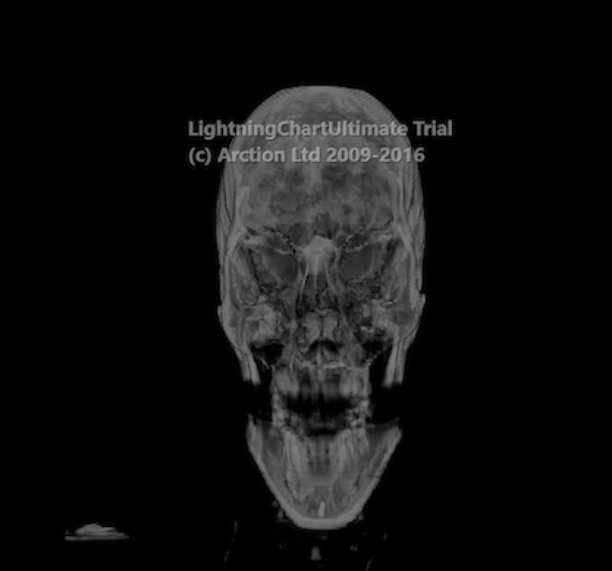
\includegraphics[scale = 0.6]{img/accum}}
\caption{An example of an accomulation function output\label{fig:accum}}
\end{figure}

Maximum intensity function visualizes only the brightest value sampled by the ray. It gives very similar results to the X-ray images. The ray function is very similar to the previous one. It is also used for-loop and step vector to sample the dataset, but it does not accumulate the information as it is done in the previous example. Instead, it keeps the biggest value which ray meets during the travel and put it to the pixel in the end. It allows end user to identify specific structures inside the volume. An example of the ray function result is shown in the figure \ref{fig:maxi}

\begin{figure}[!h]
\centerline{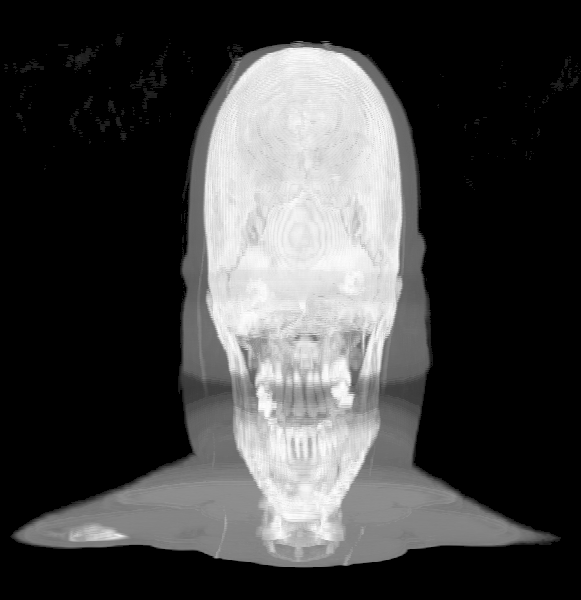
\includegraphics[scale = 0.6]{img/maxi}}
\caption{An example of maximum intensity function output\label{fig:maxi}}
\end{figure}


%https://graphics.ethz.ch/teaching/former/scivis_07/Notes/Handouts/03-raycasting.pdf



\chapter{Conclusion}
\section{Results}
\subsection{Rotation and position}
\subsection{Settings}
\subsubsection{Windowing}
\subsubsection{Thresholding}
\subsubsection{Slice range clipping}
\subsection{Mouse picking}

\section{Disscusion}

\section{Future Development}

\chapter{REFERENCES}

\chapter{Appendix}








\end{document}
